\documentclass{standalone}
\usepackage{tikz}
\usetikzlibrary{patterns, positioning}

\begin{document}
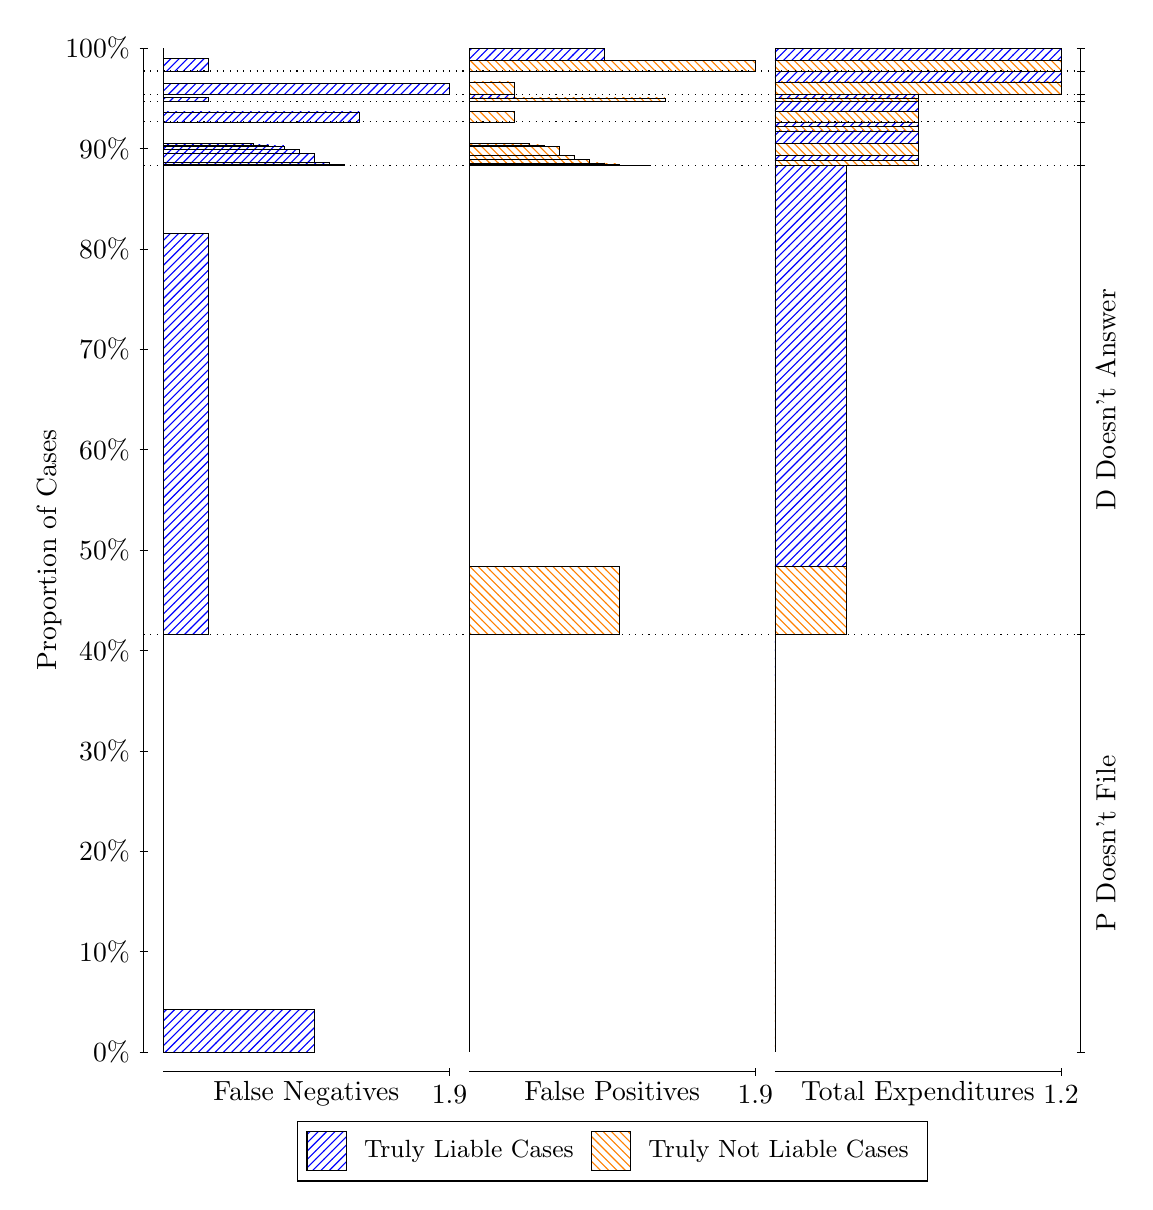
\begin{tikzpicture}
\draw[black, very thin] (1.5,1.75) -- (1.5,14.5);
\node[rotate=90, anchor=center] at (0.3, 8.125) {Proportion of Cases};
\draw[black, very thin] (1.45,1.75) -- (1.55,1.75);
\node[anchor=east] at (1.45, 1.75) {0\%};
\draw[black, very thin] (1.45,3.025) -- (1.55,3.025);
\node[anchor=east] at (1.45, 3.025) {10\%};
\draw[black, very thin] (1.45,4.3) -- (1.55,4.3);
\node[anchor=east] at (1.45, 4.3) {20\%};
\draw[black, very thin] (1.45,5.575) -- (1.55,5.575);
\node[anchor=east] at (1.45, 5.575) {30\%};
\draw[black, very thin] (1.45,6.85) -- (1.55,6.85);
\node[anchor=east] at (1.45, 6.85) {40\%};
\draw[black, very thin] (1.45,8.125) -- (1.55,8.125);
\node[anchor=east] at (1.45, 8.125) {50\%};
\draw[black, very thin] (1.45,9.4) -- (1.55,9.4);
\node[anchor=east] at (1.45, 9.4) {60\%};
\draw[black, very thin] (1.45,10.675) -- (1.55,10.675);
\node[anchor=east] at (1.45, 10.675) {70\%};
\draw[black, very thin] (1.45,11.95) -- (1.55,11.95);
\node[anchor=east] at (1.45, 11.95) {80\%};
\draw[black, very thin] (1.45,13.225) -- (1.55,13.225);
\node[anchor=east] at (1.45, 13.225) {90\%};
\draw[black, very thin] (1.45,14.5) -- (1.55,14.5);
\node[anchor=east] at (1.45, 14.5) {100\%};

\draw[black, very thin] (13.4,1.75) -- (13.4,14.5);
\draw[black, very thin] (13.35,1.75) -- (13.45,1.75);
\node[anchor=west] at (13.35, 1.75) {};
\draw[black, very thin] (13.35,7.0516) -- (13.45,7.0516);
\node[anchor=west] at (13.35, 7.0516) {};
\draw[black, very thin] (13.35,13.012) -- (13.45,13.012);
\node[anchor=west] at (13.35, 13.012) {};
\draw[black, very thin] (13.35,13.562) -- (13.45,13.562);
\node[anchor=west] at (13.35, 13.562) {};
\draw[black, very thin] (13.35,13.824) -- (13.45,13.824);
\node[anchor=west] at (13.35, 13.824) {};
\draw[black, very thin] (13.35,13.911) -- (13.45,13.911);
\node[anchor=west] at (13.35, 13.911) {};
\draw[black, very thin] (13.35,14.208) -- (13.45,14.208);
\node[anchor=west] at (13.35, 14.208) {};
\draw[black, very thin] (13.35,14.5) -- (13.45,14.5);
\node[anchor=west] at (13.35, 14.5) {};

\draw[black, very thin, pattern color=blue, pattern=north east lines] (1.75,1.75) rectangle (3.6623,2.2912);
\draw[black, very thin, pattern color=orange, pattern=north west lines] (1.75,2.2912) rectangle (1.75,7.0516);
\draw[black, very thin, pattern color=blue, pattern=north east lines] (1.75,7.0516) rectangle (2.3237,12.147);
\draw[black, very thin, pattern color=orange, pattern=north west lines] (1.75,12.147) rectangle (1.75,13.012);
\draw[black, very thin, pattern color=blue, pattern=north east lines] (1.75,13.012) rectangle (4.0447,13.027);
\draw[black, very thin, pattern color=blue, pattern=north east lines] (1.75,13.027) rectangle (3.8535,13.045);
\draw[black, very thin, pattern color=blue, pattern=north east lines] (1.75,13.045) rectangle (3.6623,13.164);
\draw[black, very thin, pattern color=blue, pattern=north east lines] (1.75,13.164) rectangle (3.4711,13.167);
\draw[black, very thin, pattern color=blue, pattern=north east lines] (1.75,13.167) rectangle (3.4711,13.212);
\draw[black, very thin, pattern color=blue, pattern=north east lines] (1.75,13.212) rectangle (3.2798,13.256);
\draw[black, very thin, pattern color=blue, pattern=north east lines] (1.75,13.256) rectangle (3.0886,13.269);
\draw[black, very thin, pattern color=blue, pattern=north east lines] (1.75,13.269) rectangle (2.8974,13.285);
\draw[black, very thin, pattern color=blue, pattern=north east lines] (1.75,13.285) rectangle (2.7061,13.286);
\draw[black, very thin, pattern color=blue, pattern=north east lines] (1.75,13.286) rectangle (2.5149,13.286);
\draw[black, very thin, pattern color=orange, pattern=north west lines] (1.75,13.286) rectangle (1.75,13.562);
\draw[black, very thin, pattern color=blue, pattern=north east lines] (1.75,13.562) rectangle (4.236,13.688);
\draw[black, very thin, pattern color=orange, pattern=north west lines] (1.75,13.688) rectangle (1.75,13.824);
\draw[black, very thin, pattern color=blue, pattern=north east lines] (1.75,13.824) rectangle (2.3237,13.87);
\draw[black, very thin, pattern color=orange, pattern=north west lines] (1.75,13.87) rectangle (1.75,13.911);
\draw[black, very thin, pattern color=blue, pattern=north east lines] (1.75,13.911) rectangle (5.3833,14.048);
\draw[black, very thin, pattern color=orange, pattern=north west lines] (1.75,14.048) rectangle (1.75,14.208);
\draw[black, very thin, pattern color=blue, pattern=north east lines] (1.75,14.208) rectangle (2.3237,14.364);
\draw[black, very thin, pattern color=orange, pattern=north west lines] (1.75,14.364) rectangle (1.75,14.5);
\draw[black, very thin, pattern color=orange, pattern=north west lines] (5.6333,1.75) rectangle (5.6333,6.5104);
\draw[black, very thin, pattern color=blue, pattern=north east lines] (5.6333,6.5104) rectangle (5.6333,7.0516);
\draw[black, very thin, pattern color=orange, pattern=north west lines] (5.6333,7.0516) rectangle (7.5456,7.9166);
\draw[black, very thin, pattern color=blue, pattern=north east lines] (5.6333,7.9166) rectangle (5.6333,13.012);
\draw[black, very thin, pattern color=orange, pattern=north west lines] (5.6333,13.012) rectangle (7.9281,13.013);
\draw[black, very thin, pattern color=orange, pattern=north west lines] (5.6333,13.013) rectangle (7.7368,13.013);
\draw[black, very thin, pattern color=orange, pattern=north west lines] (5.6333,13.013) rectangle (7.5456,13.029);
\draw[black, very thin, pattern color=orange, pattern=north west lines] (5.6333,13.029) rectangle (7.3544,13.042);
\draw[black, very thin, pattern color=orange, pattern=north west lines] (5.6333,13.042) rectangle (7.1632,13.086);
\draw[black, very thin, pattern color=orange, pattern=north west lines] (5.6333,13.086) rectangle (6.9719,13.134);
\draw[black, very thin, pattern color=orange, pattern=north west lines] (5.6333,13.134) rectangle (6.7807,13.253);
\draw[black, very thin, pattern color=orange, pattern=north west lines] (5.6333,13.253) rectangle (6.5895,13.271);
\draw[black, very thin, pattern color=orange, pattern=north west lines] (5.6333,13.271) rectangle (6.3982,13.288);
\draw[black, very thin, pattern color=blue, pattern=north east lines] (5.6333,13.288) rectangle (6.0158,13.289);
\draw[black, very thin, pattern color=blue, pattern=north east lines] (5.6333,13.289) rectangle (5.8246,13.29);
\draw[black, very thin, pattern color=blue, pattern=north east lines] (5.6333,13.29) rectangle (5.6333,13.562);
\draw[black, very thin, pattern color=orange, pattern=north west lines] (5.6333,13.562) rectangle (6.207,13.699);
\draw[black, very thin, pattern color=blue, pattern=north east lines] (5.6333,13.699) rectangle (5.6333,13.824);
\draw[black, very thin, pattern color=orange, pattern=north west lines] (5.6333,13.824) rectangle (8.1193,13.866);
\draw[black, very thin, pattern color=blue, pattern=north east lines] (5.6333,13.866) rectangle (6.207,13.911);
\draw[black, very thin, pattern color=orange, pattern=north west lines] (5.6333,13.911) rectangle (6.207,14.07);
\draw[black, very thin, pattern color=blue, pattern=north east lines] (5.6333,14.07) rectangle (5.6333,14.208);
\draw[black, very thin, pattern color=orange, pattern=north west lines] (5.6333,14.208) rectangle (9.2667,14.344);
\draw[black, very thin, pattern color=blue, pattern=north east lines] (5.6333,14.344) rectangle (7.3544,14.5);
\draw[black, very thin, pattern color=orange, pattern=north west lines] (9.5167,1.75) rectangle (9.5167,6.5104);
\draw[black, very thin, pattern color=blue, pattern=north east lines] (9.5167,6.5104) rectangle (9.5167,7.0516);
\draw[black, very thin, pattern color=orange, pattern=north west lines] (9.5167,7.0516) rectangle (10.425,7.9166);
\draw[black, very thin, pattern color=blue, pattern=north east lines] (9.5167,7.9166) rectangle (10.425,13.012);
\draw[black, very thin, pattern color=orange, pattern=north west lines] (9.5167,13.012) rectangle (11.333,13.073);
\draw[black, very thin, pattern color=blue, pattern=north east lines] (9.5167,13.073) rectangle (11.333,13.135);
\draw[black, very thin, pattern color=orange, pattern=north west lines] (9.5167,13.135) rectangle (11.333,13.293);
\draw[black, very thin, pattern color=blue, pattern=north east lines] (9.5167,13.293) rectangle (11.333,13.448);
\draw[black, very thin, pattern color=orange, pattern=north west lines] (9.5167,13.448) rectangle (11.333,13.505);
\draw[black, very thin, pattern color=blue, pattern=north east lines] (9.5167,13.505) rectangle (11.333,13.562);
\draw[black, very thin, pattern color=orange, pattern=north west lines] (9.5167,13.562) rectangle (11.333,13.699);
\draw[black, very thin, pattern color=blue, pattern=north east lines] (9.5167,13.699) rectangle (11.333,13.824);
\draw[black, very thin, pattern color=orange, pattern=north west lines] (9.5167,13.824) rectangle (11.333,13.866);
\draw[black, very thin, pattern color=blue, pattern=north east lines] (9.5167,13.866) rectangle (11.333,13.911);
\draw[black, very thin, pattern color=orange, pattern=north west lines] (9.5167,13.911) rectangle (13.15,14.07);
\draw[black, very thin, pattern color=blue, pattern=north east lines] (9.5167,14.07) rectangle (13.15,14.208);
\draw[black, very thin, pattern color=orange, pattern=north west lines] (9.5167,14.208) rectangle (13.15,14.344);
\draw[black, very thin, pattern color=blue, pattern=north east lines] (9.5167,14.344) rectangle (13.15,14.5);
\draw[black, dotted] (1.5,7.0516) -- (13.4,7.0516);
\draw[black, dotted] (1.5,13.012) -- (13.4,13.012);
\draw[black, dotted] (1.5,13.562) -- (13.4,13.562);
\draw[black, dotted] (1.5,13.824) -- (13.4,13.824);
\draw[black, dotted] (1.5,13.911) -- (13.4,13.911);
\draw[black, dotted] (1.5,14.208) -- (13.4,14.208);
\draw[black, very thin] (1.75,1.5) -- (5.3833,1.5);
\node[anchor=north] at (3.5667, 1.5) {False Negatives};
\draw[black, very thin] (5.3833,1.45) -- (5.3833,1.55);
\node[anchor=north] at (5.3833, 1.45) {1.9};

\draw[black, very thin] (5.6333,1.5) -- (9.2667,1.5);
\node[anchor=north] at (7.45, 1.5) {False Positives};
\draw[black, very thin] (9.2667,1.45) -- (9.2667,1.55);
\node[anchor=north] at (9.2667, 1.45) {1.9};

\draw[black, very thin] (9.5167,1.5) -- (13.15,1.5);
\node[anchor=north] at (11.333, 1.5) {Total Expenditures};
\draw[black, very thin] (13.15,1.45) -- (13.15,1.55);
\node[anchor=north] at (13.15, 1.45) {1.2};

\node[black, centered, rotate=90] at (13.72, 4.4008) {P Doesn't File};
\node[black, centered, rotate=90] at (13.72, 10.032) {D Doesn't Answer};






\draw (7.449999999999999,1.5) node[draw=none] (baseCoordinate) {};
\begin{scope}[align=center]
        \matrix[scale=0.5, draw=black, below=0.5cm of baseCoordinate, nodes={draw}, column sep=0.1cm]{
            \node[rectangle, draw, minimum width=0.5cm, minimum height=0.5cm, pattern=north east lines, pattern color=blue] {}; &
            \node[draw=none, font=\small] (B) {Truly Liable Cases}; &
            \node[rectangle, draw, minimum width=0.5cm, minimum height=0.5cm, pattern=north west lines, pattern color=orange] {}; &
            \node[draw=none, font=\small] (B) {Truly Not Liable Cases}; \\
            };
\end{scope}

\end{tikzpicture}
\end{document}